\chapter{Demo}
Demo link\footnote{Only available for certain time}: \url{https://github.com/rdmorgnzation/soilbearing}\\

Program Tabs, screenshots and info\\
==========
Program has theme selection, so screenshots are diffrents.\\
\textbf{Start Screen}\\
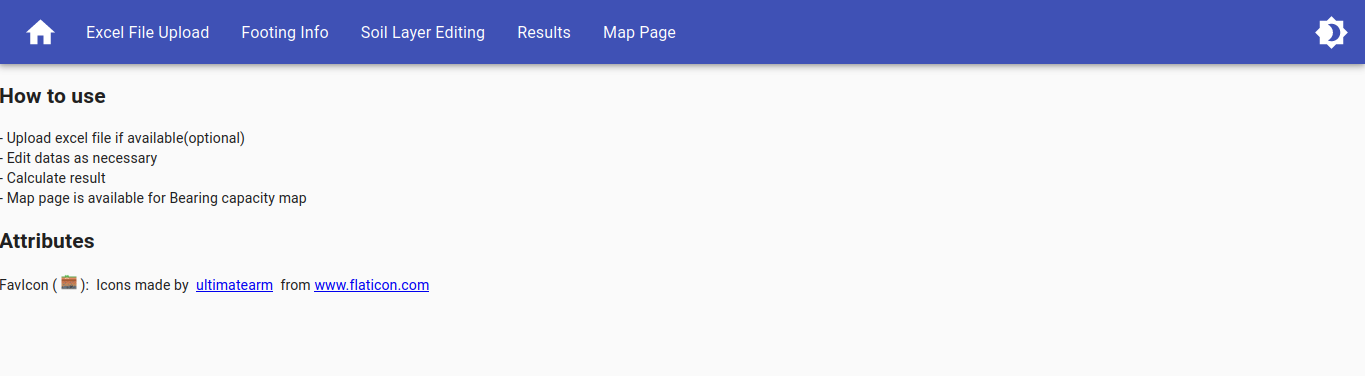
\includegraphics[width=\linewidth,keepaspectratio]{../proj/soilbearing/media/images/index.png}
General info about program\\

\textbf{Upload Tab}\\
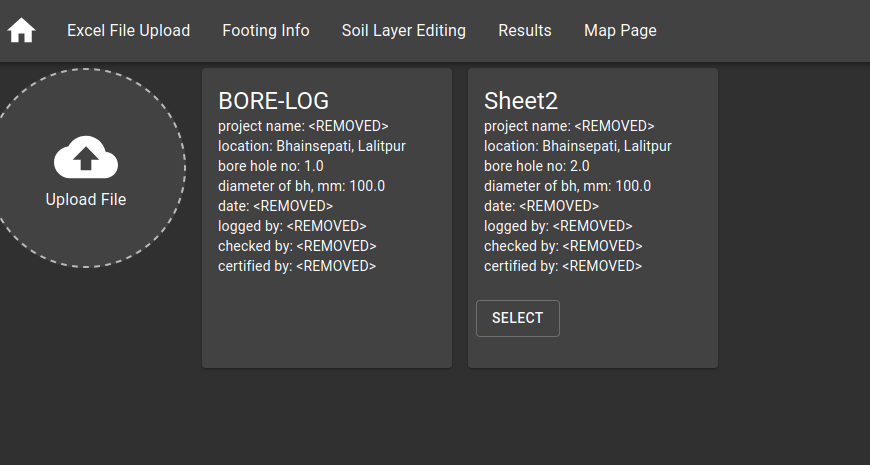
\includegraphics[width=\linewidth,keepaspectratio]{../proj/soilbearing/media/images/fileInfo.png}
Upload the excel file. (either .xls, or .xlsx)\\
If more than one sheet is available in file then sheet selection option.\\
\begin{itemize}
\item Click and select, or\\
\item drag and drop\\
\end{itemize}

\textbf{Footing info Tab}\\
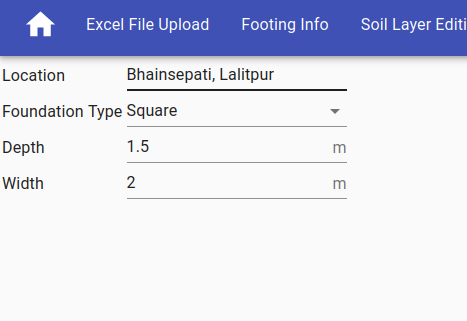
\includegraphics[width=\linewidth,keepaspectratio]{../proj/soilbearing/media/images/footing_info.png}
Basic footing info,\\

\textbf{Edit Tab}
There are 2 modes:-\\
\textbf{Edit Mode}\\
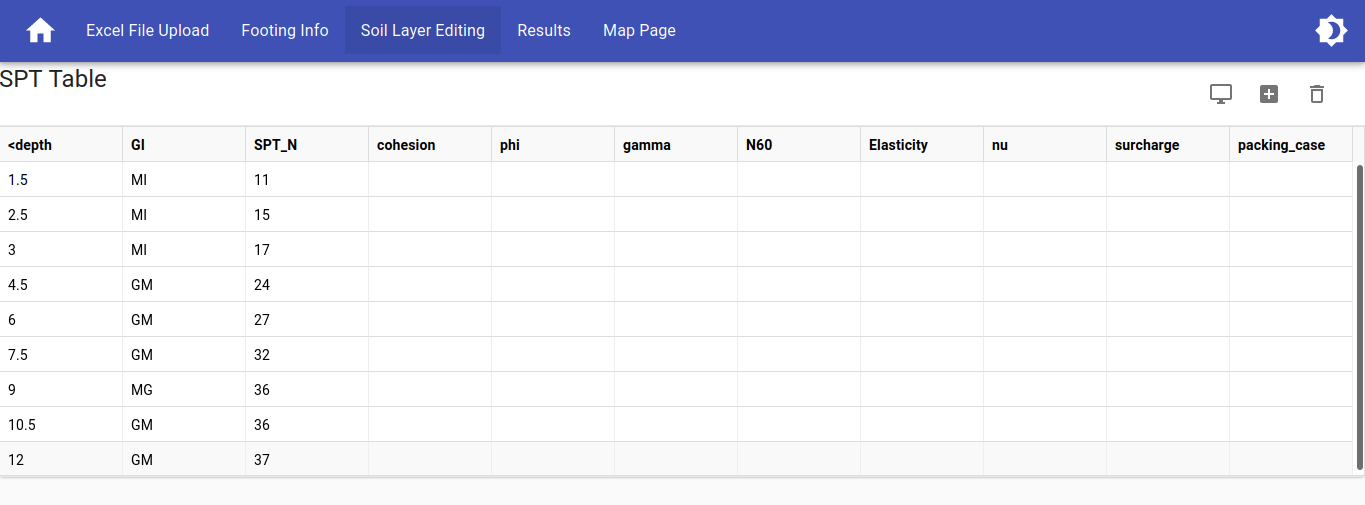
\includegraphics[width=\linewidth,keepaspectratio]{../proj/soilbearing/media/images/edit_mode.png}
Actual editing\\

\textbf{Preview Mode}\\
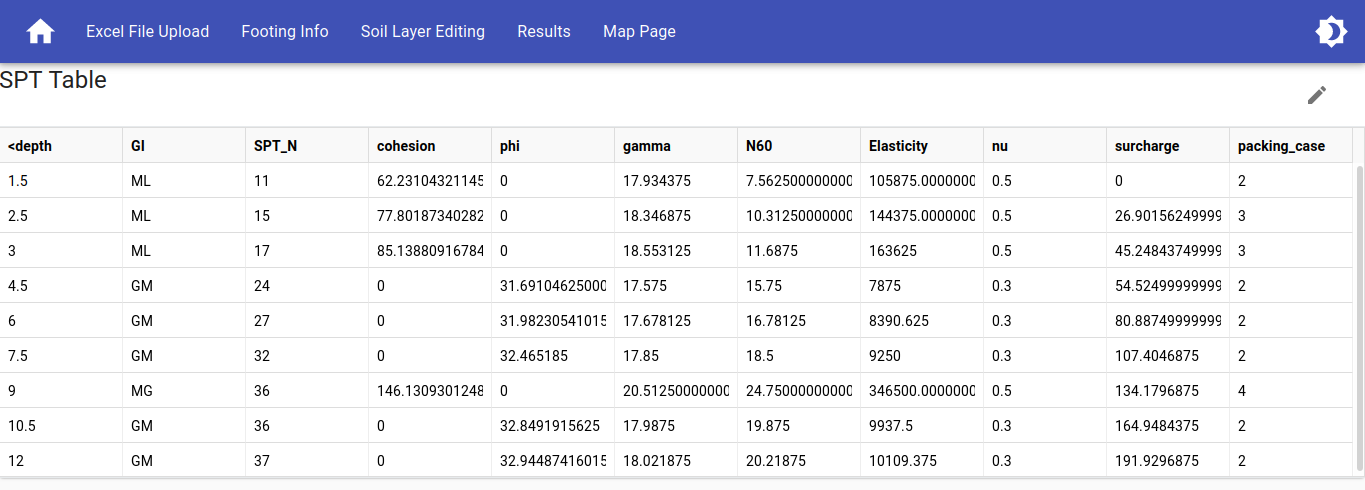
\includegraphics[width=\linewidth,keepaspectratio]{../proj/soilbearing/media/images/preview_mode.png}
See program internal interpolations, etc. \\

\textbf{Results Tab}\\
There are 2 options:-\\
\textbf{From datas as above}\\
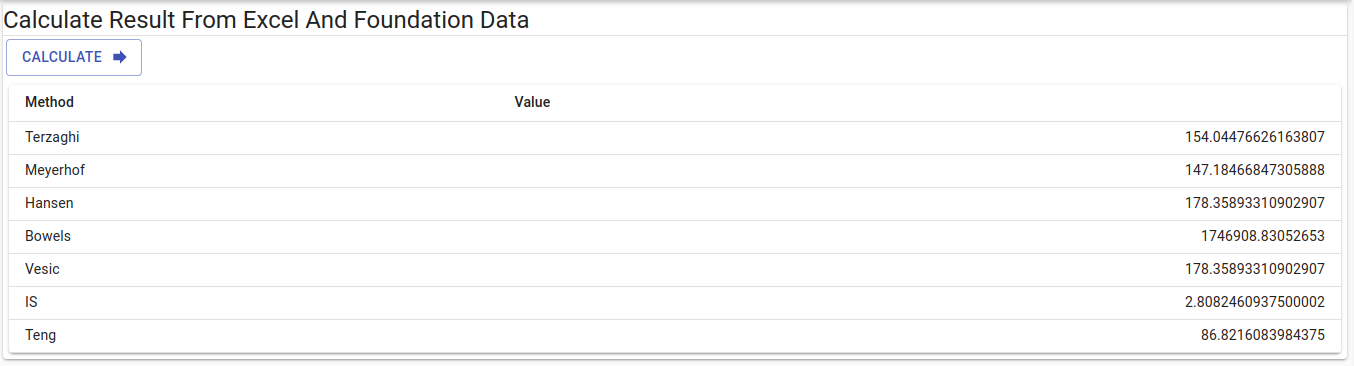
\includegraphics[width=\linewidth,keepaspectratio]{../proj/soilbearing/media/images/fed.png}
Calculation as per above datas.\\

\textbf{Calculate from Interpolation}\\
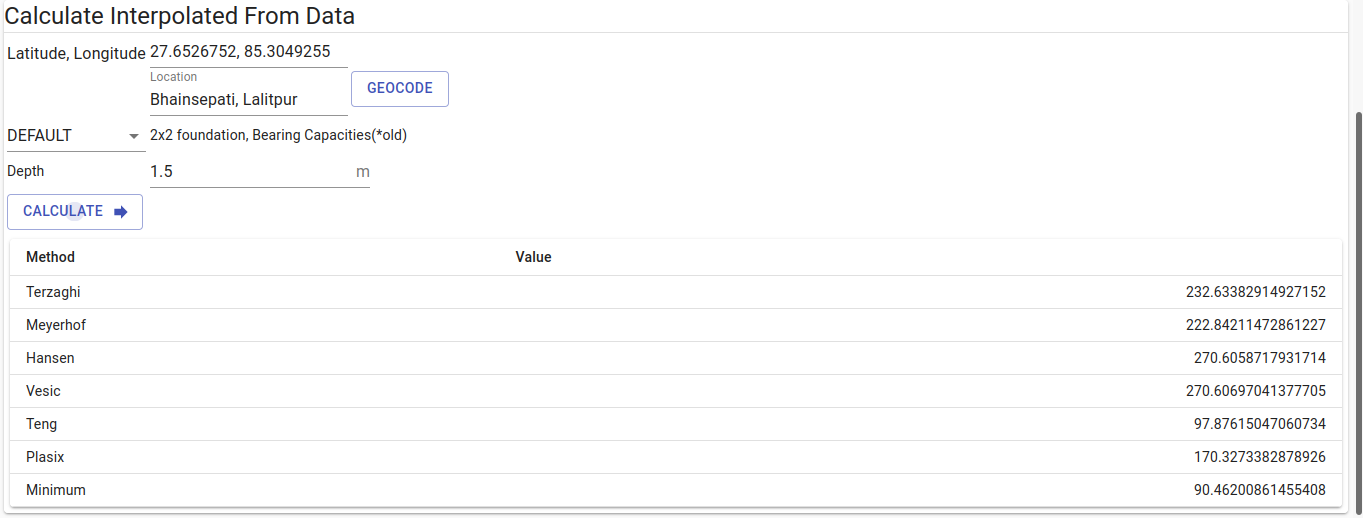
\includegraphics[width=\linewidth,keepaspectratio]{../proj/soilbearing/media/images/ID.png}
Datas interpolated by IDW from the project report datas.\\
Geocode from name, to get latitude and longitude.\\

\textbf{Map Tab}\\
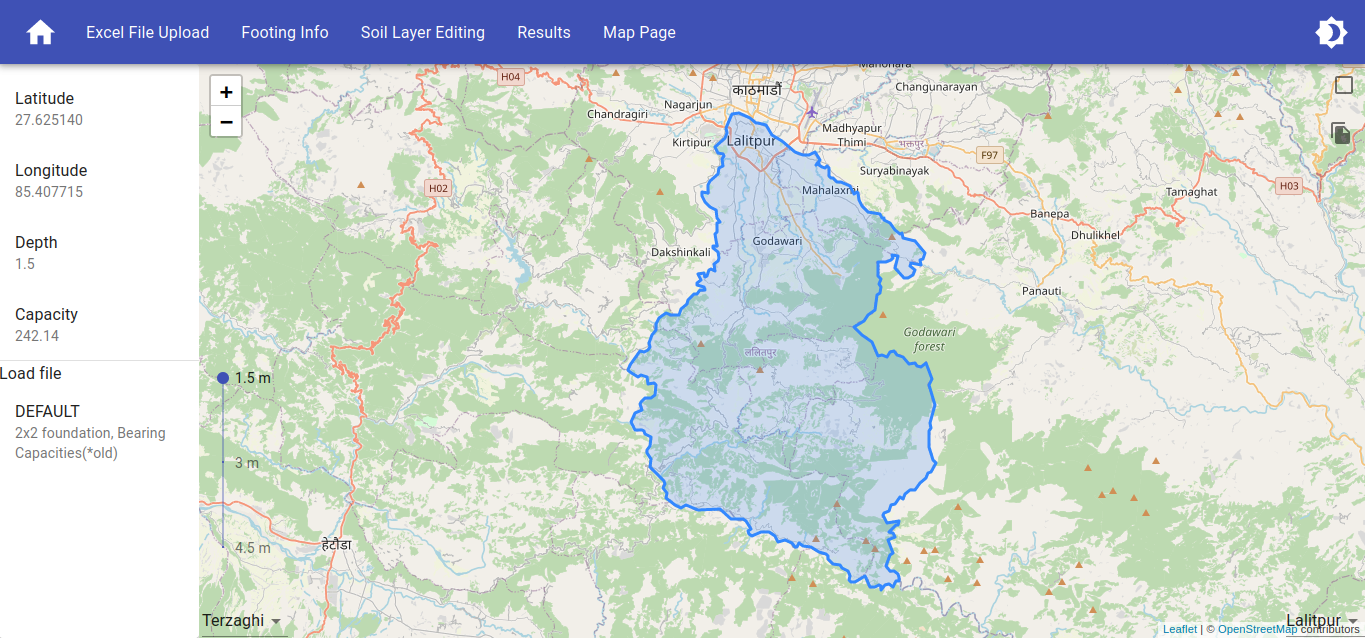
\includegraphics[width=\linewidth,keepaspectratio]{../proj/soilbearing/media/images/map_page.png}
Map from datas computed by interpolation.\\